\section{Experimental Evaluation}
\label{sect:experimental-evaluation}

We create various plots showing the distribution of the maps' qualities to gain insights into the effect of the number of clusters $n$, the nesting ratio $\alpha$, nesting bias $\beta$, and the number of dynamic operations $t$ on the different quality metrics.
In these plots, we vary the value for one of these parameters, while keeping the others constant.

\Cref{fig:experimental-evaluation-variable-number-of-operations} shows how the number of dynamic operations $t$ applied to the instance affects the cartographic error and polygon complexity.

\begin{figure}[H]
	\centering
	\subfigure{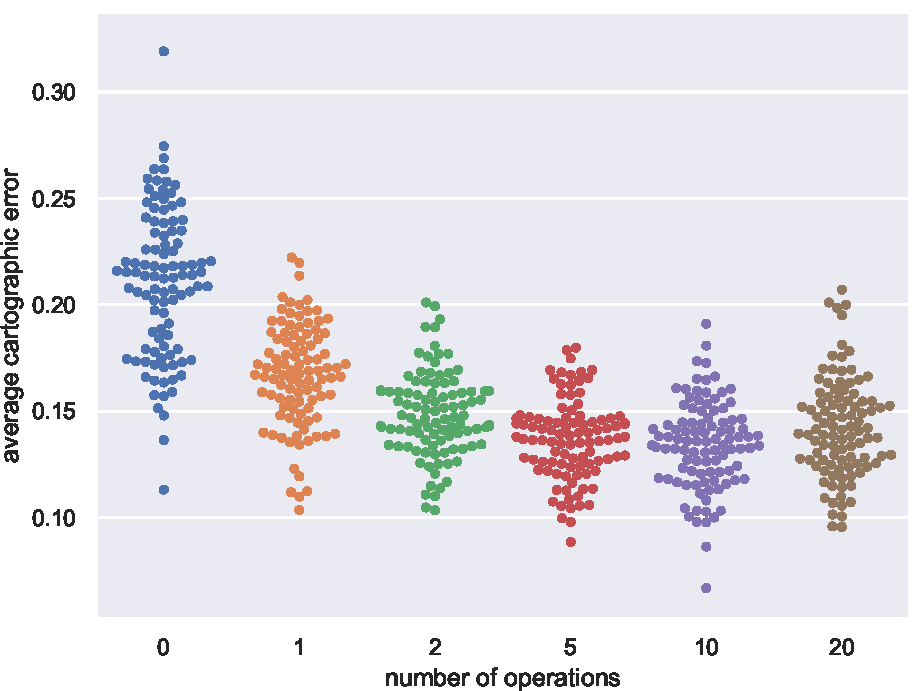
\includegraphics[width=0.47\textwidth]{Resources/Evaluation-AverageCartographicError-t.pdf}}
	\quad
	\subfigure{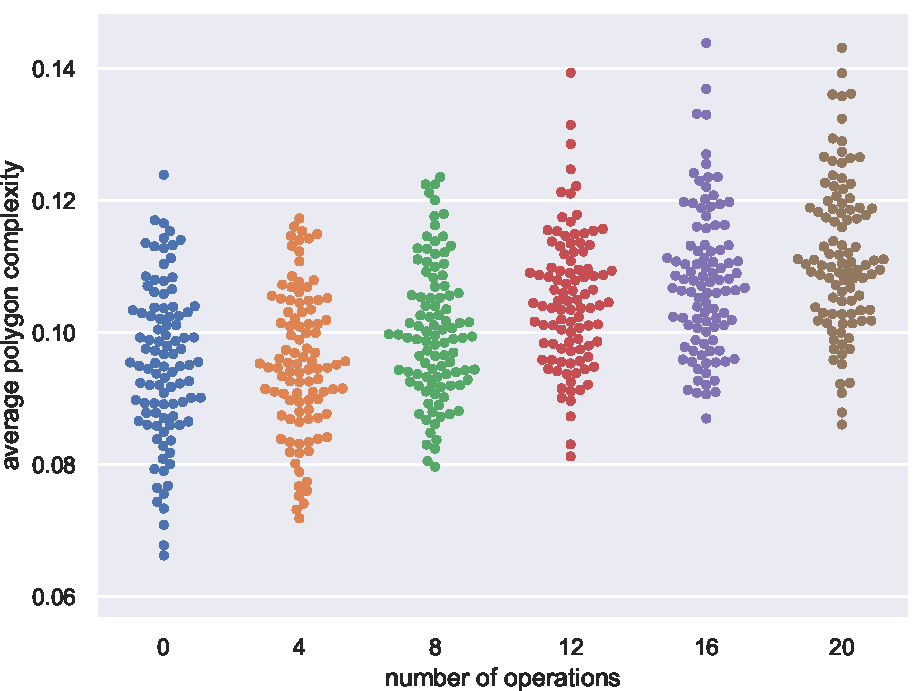
\includegraphics[width=0.47\textwidth]{Resources/Evaluation-AveragePolygonComplexity-t.pdf}}
	\subfigure{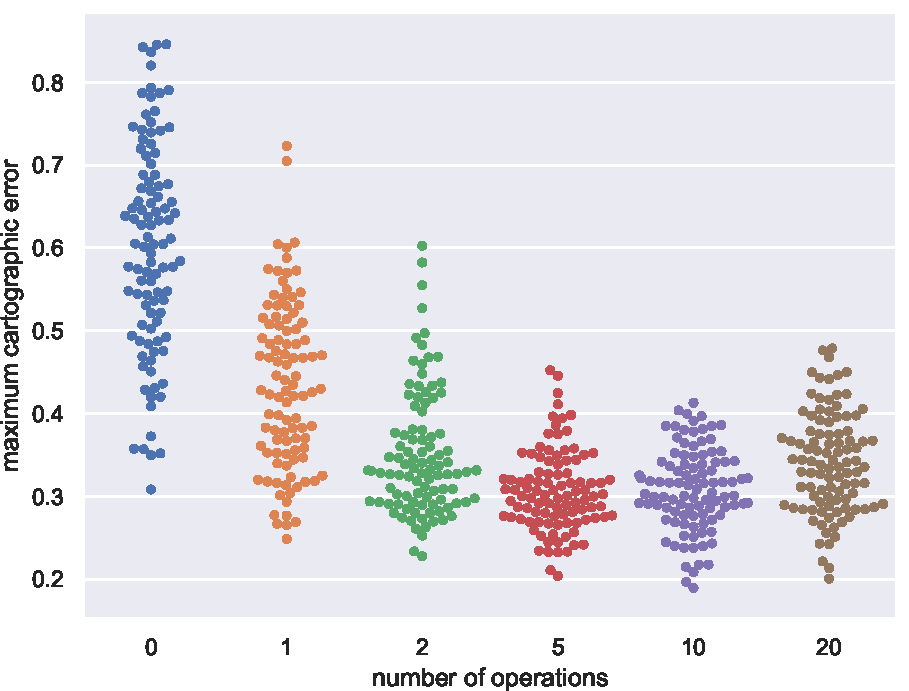
\includegraphics[width=0.47\textwidth]{Resources/Evaluation-MaximumCartographicError-t.pdf}}
	\quad
	\subfigure{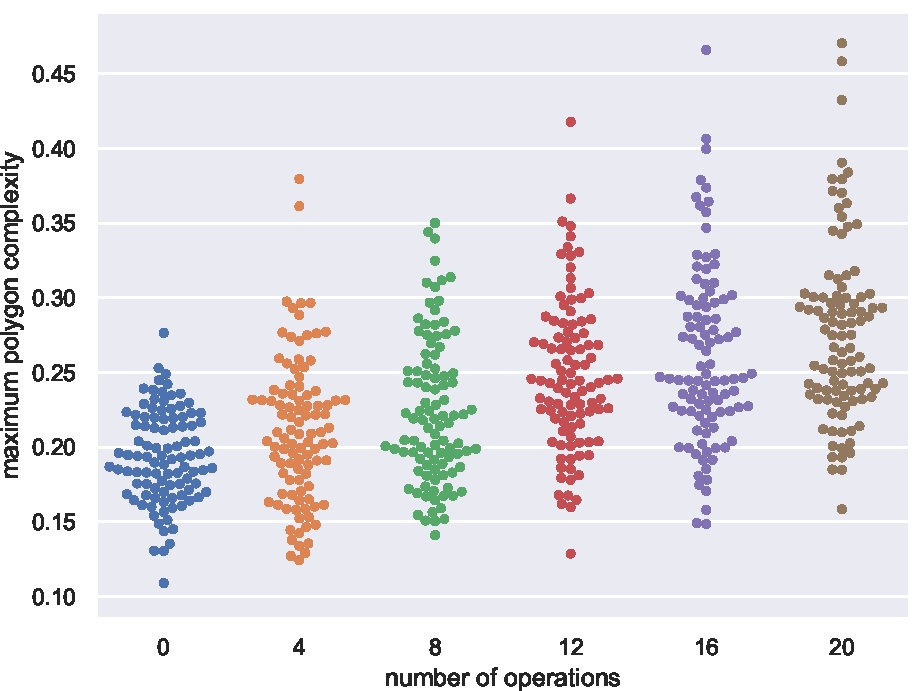
\includegraphics[width=0.47\textwidth]{Resources/Evaluation-MaximumPolygonComplexity-t.pdf}}
	\caption{Quality metrics of maps \propmap{t} for 100 randomized instances after applying a different number of operations $t$, with $n = 20$, $\alpha = 0$, and $\beta = 0$.}
	\label{fig:experimental-evaluation-variable-number-of-operations}
\end{figure}

We can see that as we apply more operations, the cartographic error decreases, and very quickly so: after $t = 5$ operations, the cartographic errors become almost indistinguishable.
We believe that this is because, for larger values of $t$, the force-directed optimization algorithm has more time overall to optimize the statistical accuracy of the maps, amongst other features.

The polygon complexity, on the other hand, increases over time.
When processing topology-altering operations, additional subdivision vertices may be inserted to prevent the introduction of edge crossings, potentially creating shapes that are not locally fat in the process.
The optimization algorithm obviously tries to improve the local fatness of the involved regions afterward.
However, it seems unable to do so until around $t = 16$, where it seems to become able to counteract these effects and to prevent further degradation.
In \cref{sect:future-work}, we discuss an approach to verify whether this change indeed happens over time, or lies in the nature of the arrangement of the regions in the different test instances.

The maximum cartographic error and polygon complexity over all regions of the map paint pictures with similar trends but greater mean and variance as outliers have a more significant impact on the map's overall quality.

\vspace{1cm}

The effect of the initial number of clusters $n$ on the maps' quality is shown in \cref{fig:experimental-evaluation-variable-number-of-vertices}.

\begin{figure}[H]
	\centering
	\subfigure{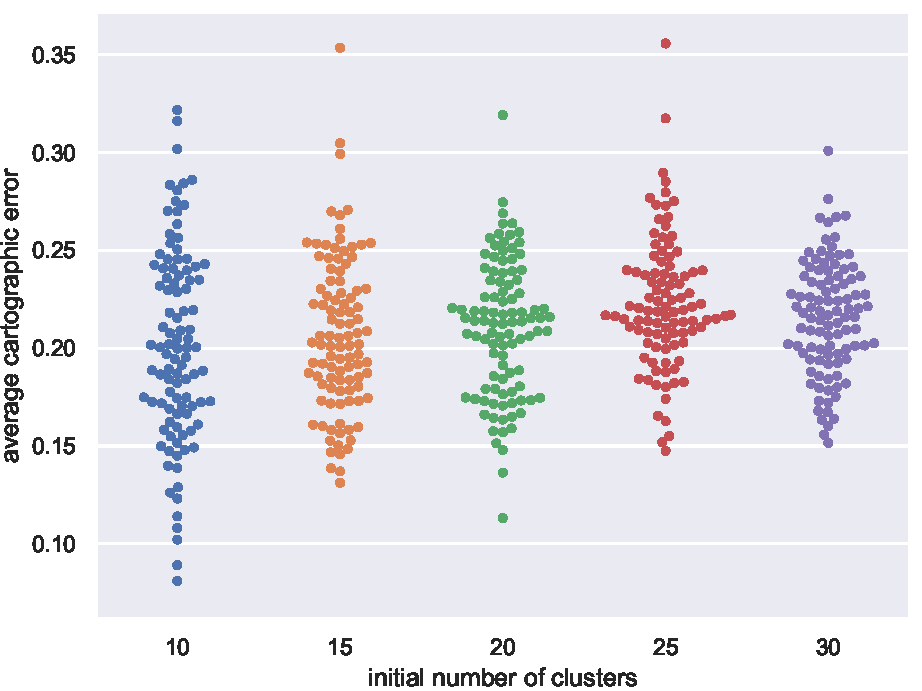
\includegraphics[width=0.47\textwidth]{Resources/Evaluation-AverageCartographicError-n.pdf}}
	\quad
	\subfigure{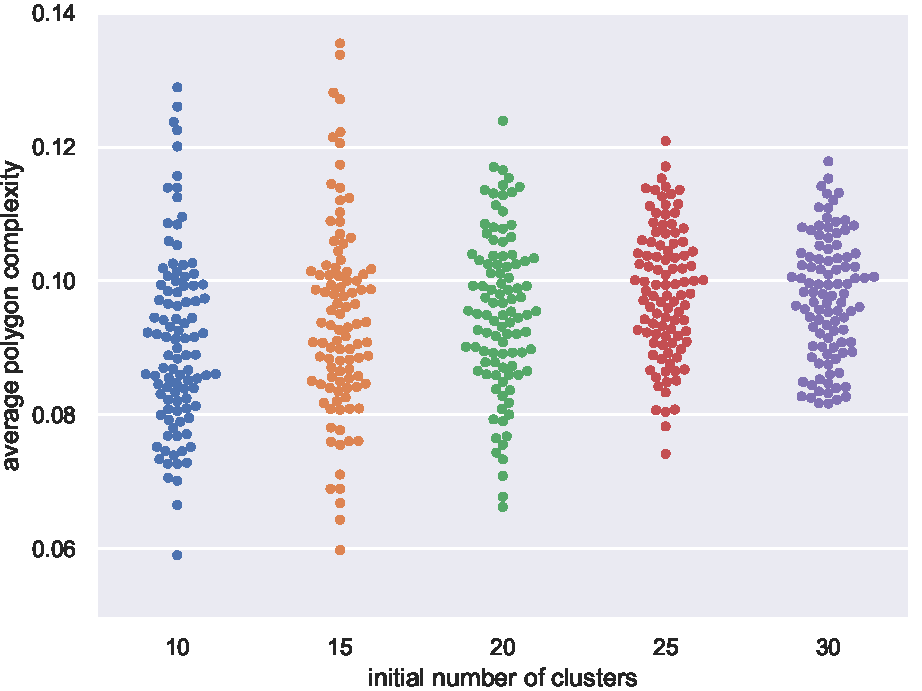
\includegraphics[width=0.47\textwidth]{Resources/Evaluation-AveragePolygonComplexity-n.pdf}}
	\subfigure{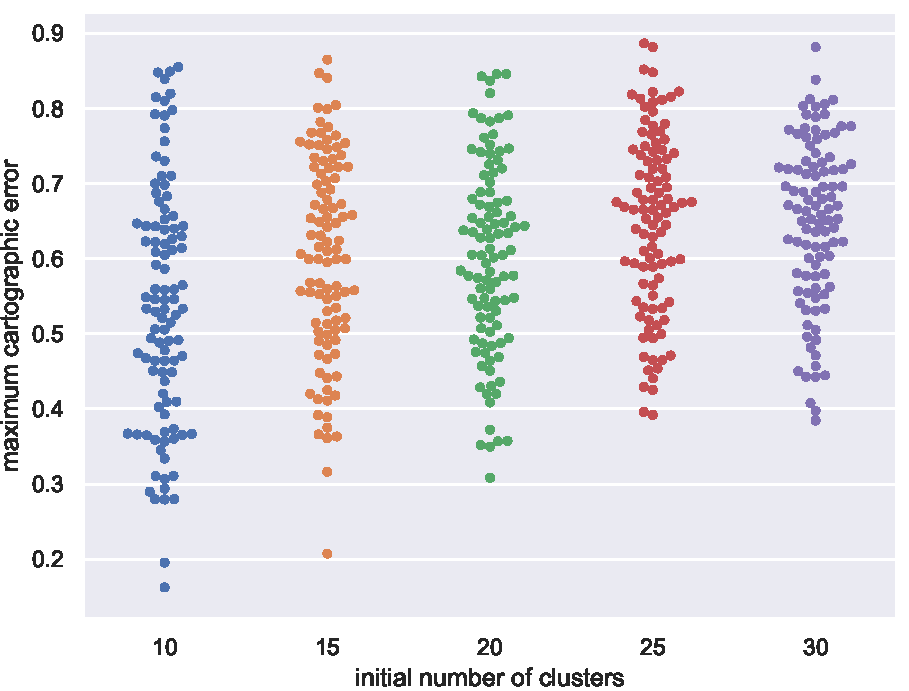
\includegraphics[width=0.47\textwidth]{Resources/Evaluation-MaximumCartographicError-n.pdf}}
	\quad
	\subfigure{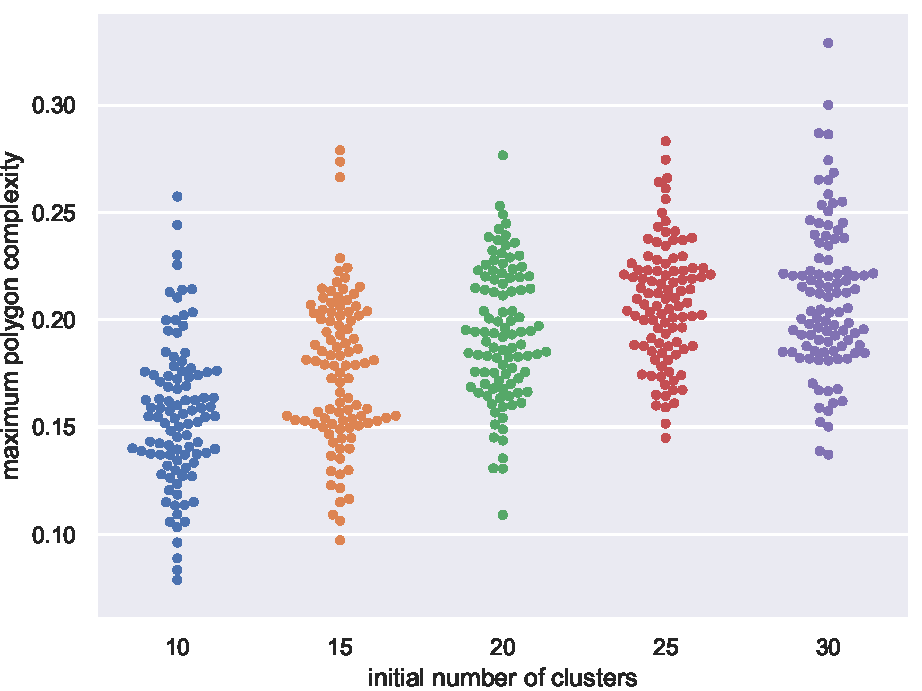
\includegraphics[width=0.47\textwidth]{Resources/Evaluation-MaximumPolygonComplexity-n.pdf}}
	\caption{Quality metrics of maps \propmap{t} for 100 randomized instances with different numbers of clusters $n$, with $\alpha = 0$, $\beta = 0$, and $t = 0$.}
	\label{fig:experimental-evaluation-variable-number-of-vertices}
\end{figure}

The average cartographic error across all instances appears mostly unaffected by the input size.
Its variance decreases, though, as we increase the number of clusters.
This observation makes sense because as there are more clusters, the impact an outlier has on the average cartographic error decreases.

Regarding the polygon complexity, a slight increase in complexity for larger input sizes can be seen in the plot.
We believe that this is because, for larger instances, there is simply more room for challenging constructs that require higher polygon complexity to visualize correctly.

With a larger number of clusters, there come more potential outliers that can negatively affect the instances' maximum cartographic errors and polygon complexities.
Hence we see more pronounced trends for these two metrics.

\clearpage

\Cref{fig:experimental-evaluation-variable-nesting-ratio-and-bias} shows the effects of different combinations of nesting ratio $\alpha$ and nesting bias $\beta$ on the maps' quality.

\begin{figure}[H]
	\centering
	\subfigure{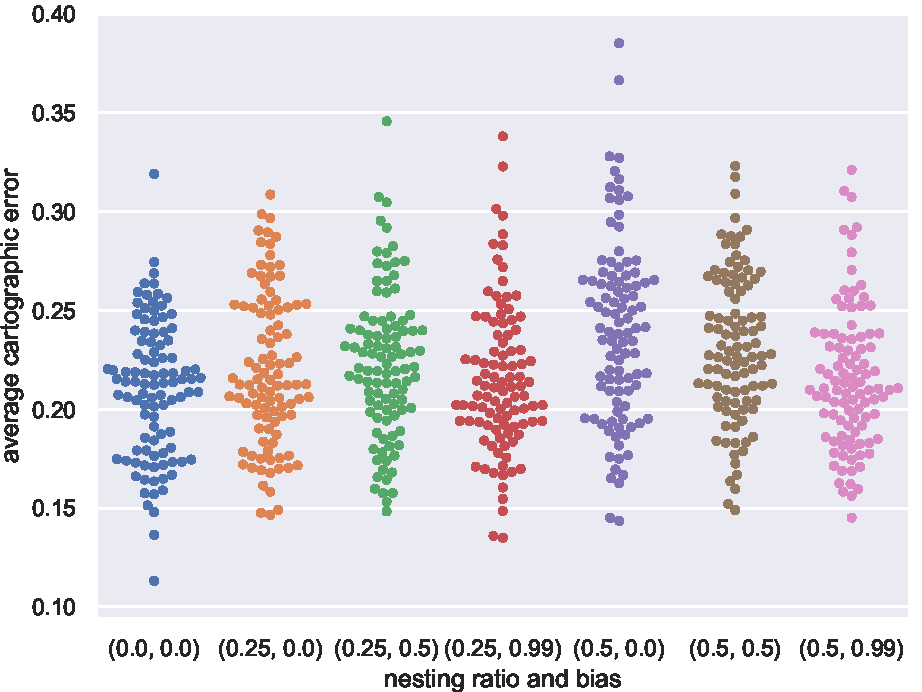
\includegraphics[width=0.47\textwidth]{Resources/Evaluation-AverageCartographicError-ab.pdf}}
	\quad
	\subfigure{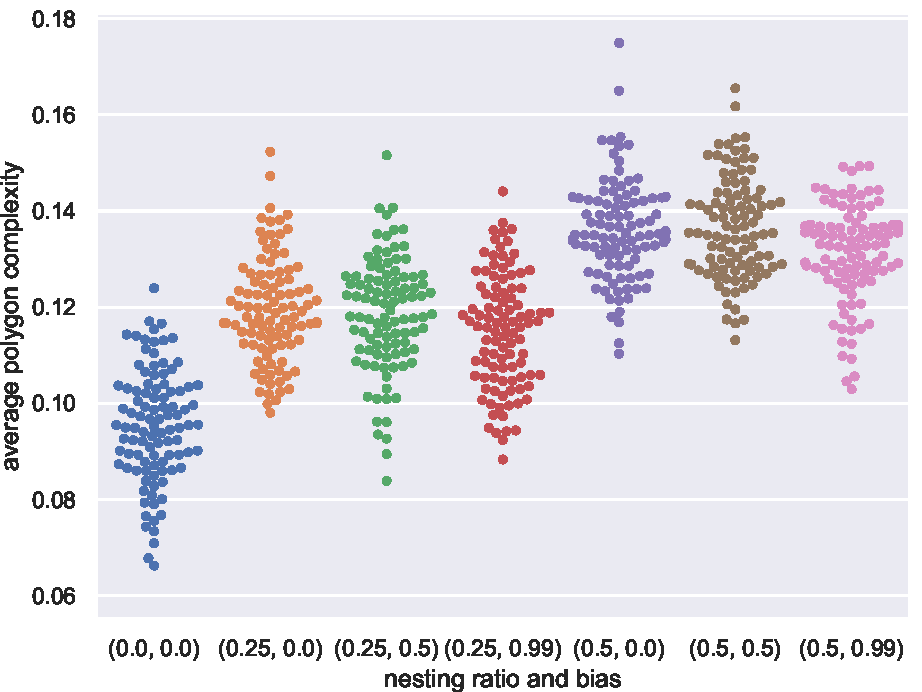
\includegraphics[width=0.47\textwidth]{Resources/Evaluation-AveragePolygonComplexity-ab.pdf}}
	\subfigure{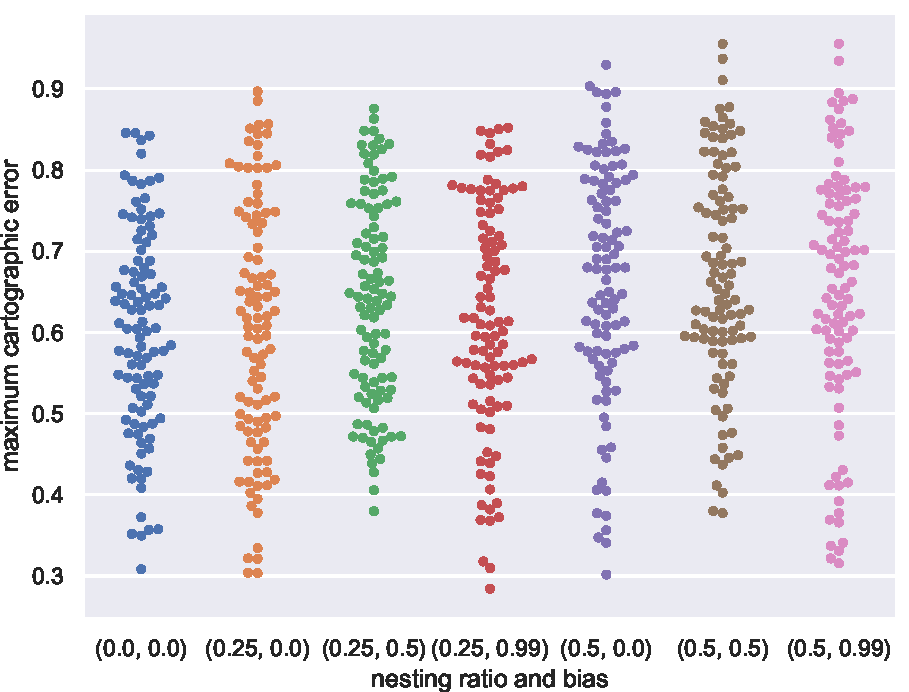
\includegraphics[width=0.47\textwidth]{Resources/Evaluation-MaximumCartographicError-ab.pdf}}
	\quad
	\subfigure{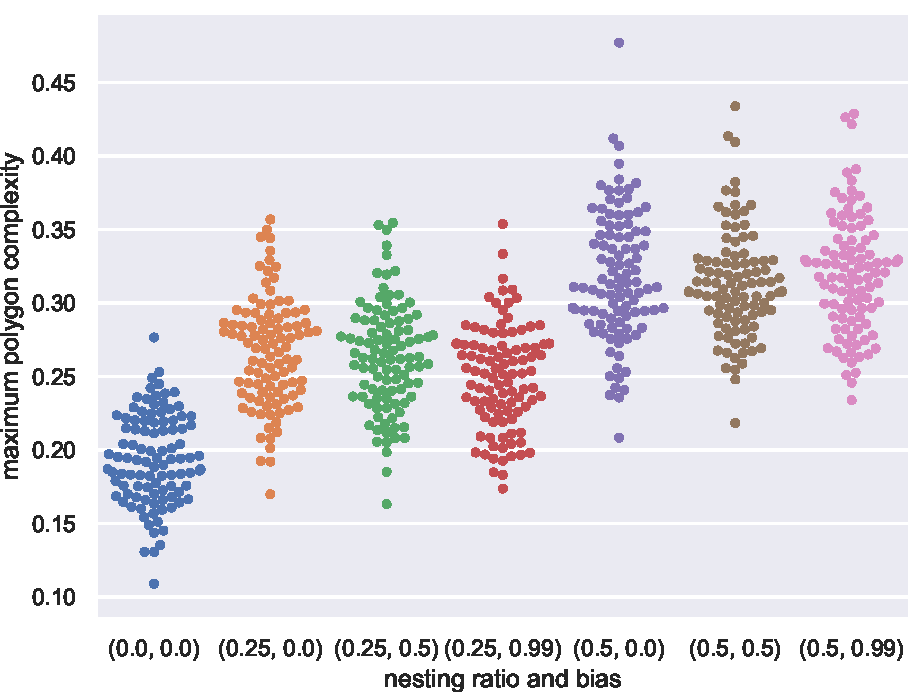
\includegraphics[width=0.47\textwidth]{Resources/Evaluation-MaximumPolygonComplexity-ab.pdf}}
	\caption{Quality metrics of maps \propmap{t} for 100 randomized instances with different nesting ratios $\alpha$ and nesting biases $\beta$, with $n = 20$ and $t = 0$.}
	\label{fig:experimental-evaluation-variable-nesting-ratio-and-bias}
\end{figure}

We cannot see any meaningful effect of nesting ratio and bias on the maps' cartographic error.

For the polygon complexity, however, the nesting ratio $\alpha$ has a pronounced impact.
The figure clearly shows that instances with $\alpha = 0.25$ tend to have higher polygon complexities than instances with $\alpha = 0$, and instances with $\alpha = 0.5$ even higher ones, regardless of nesting bias $\beta$.

A possible explanation is that by nesting vertices of the cluster graph into existing triangles, we create internal vertices with low degrees.
Therefore, the regions of the map corresponding to these vertices are surrounded by few neighboring regions, which are inevitably more complex as these few regions have to span the entire boundary of the original region.
Additionally, there generally lie fewer vertices on the outer face of the cluster graph, whose corresponding regions must again surround the entire inside.
These decreases in the number of external vertices and average degree of internal vertices as the nesting ratio $\alpha$ increases are illustrated in \cref{fig:experimental-evaluation-variable-nesting-ratio-and-bias-2}.

\begin{figure}[H]
	\centering
	\subfigure{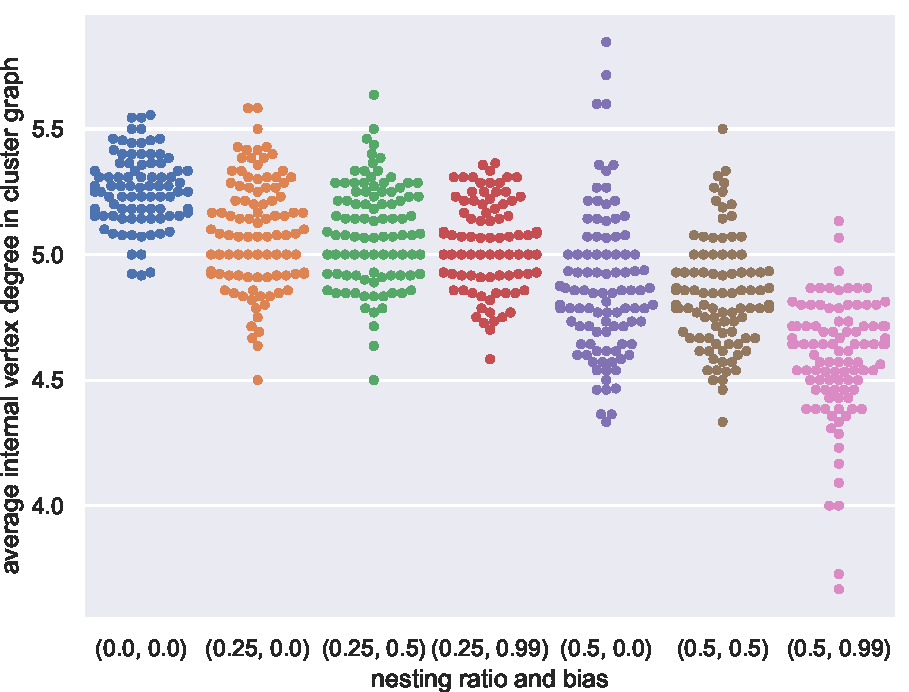
\includegraphics[width=0.47\textwidth]{Resources/Evaluation-AverageDegreeOfInternalVertices-ab.pdf}}
	\quad
	\subfigure{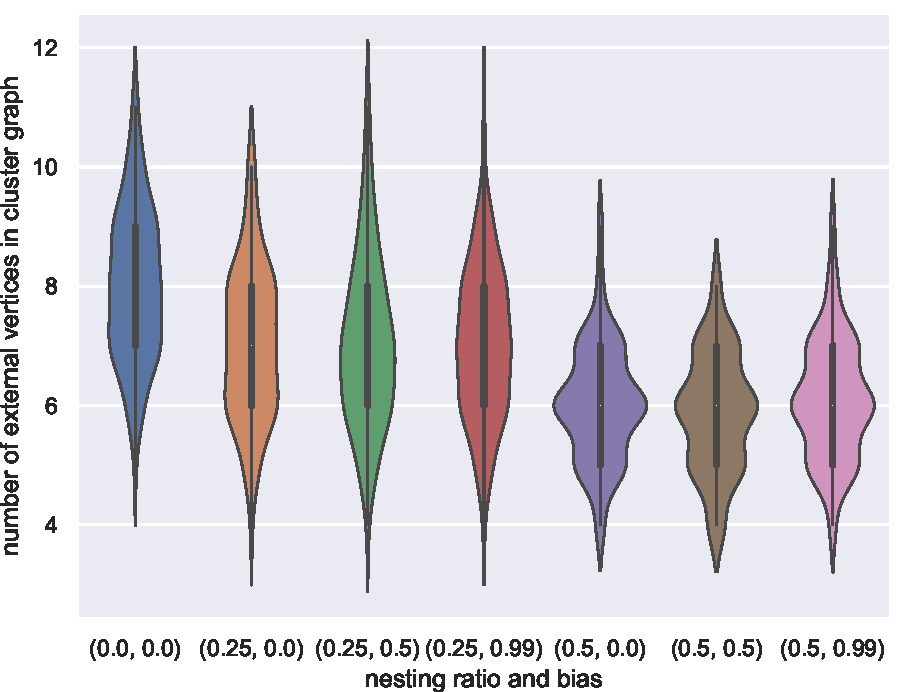
\includegraphics[width=0.47\textwidth]{Resources/Evaluation-NumberOfExternalVertices-ab.pdf}}
	\caption{Properties of 100 randomized filtered cluster graphs \clustergraph{t} with different nesting ratios $\alpha$ and nesting biases $\beta$, with $n = 20$ and $t = 0$.}
	\label{fig:experimental-evaluation-variable-nesting-ratio-and-bias-2}
\end{figure}

\Cref{fig:experimental-evaluation-variable-nesting-ratio-and-bias} also indicates that for fixed a nesting ratio $\alpha$, the nesting bias $\beta$ slightly reduces the map's polygon complexity.
However, this observation is not significant enough to jump to any conclusions.

Again, the maximum polygon complexity over all regions of the map exhibits the same overall trend but with a larger spread.
